% !TEX root = ../Geodesics_BV2.tex

\section{Numerical Computations of Geodesics}
\label{discretization}

In this section we discretize and relax problem~\eqref{problem} in order to approximate numerically  geodesic paths. Note that, since we use a gradient descent to minimize a discretized and relaxed energy, the resulting optimal discrete homotopy aims at approximating stationary points of the geodesic energy, and that these homotopies cannot be guaranteed to be globally minimizing geodesics. 


%%%%%%%%%%%%%%%%%%%%%%%%%%%%%%%%%%%%%%%%%%%%%%%%%
\subsection{Penalized Boundary Condition at $t=1$}

To obtain a simple numerical scheme, we first relax the constraint $\GA(1)=\gm_1$ by adding at the energy $E$ a data fidelity term $H(\GA(1), \gm_1)$ taking into account the deviation between $\GA(1)$ and $\gm_1$. In the following we make use of the $H$ functional defined  in~\cite[equation 5.4]{Rigid-evol} .

Such a functional is defined as the following distance between two curves

$$H(\gm,\la) = \int_{\Circ} \int_{\Circ} \|\n_{\gm}(s) - \n_{\lambda}(t)\|^2 \; 
	k\left( \gm(s) , \lambda(t) \right)\; \d \gm(s) \d \lambda(t)\; \quad 
	\forall \gm, \la \in \Bb$$
where

$$	k(v, w) =  e^{-\frac{\|v-w\|^2}{2\sigma^2}} + e^{-\frac{\|v-w\|^2}{2\delta^2} } 
	\quad \quad \forall v,\,w\in \R^2\,.
$$
Here $(\sigma,\delta)$ are positive constants that should be adapted depending on the targeted application. We use a sum of Gaussian kernels to better
capture geometric features at different scales in the curves to be matched. This has been shown to be quite
efficient in practice in a different context in \cite{FX-ref}. According to our numerical tests, the use of more than two kernels does not improve the results.

This functional $H$ was initially proposed in~\cite{currents-matching} as a norm on a reproducing Hilbert space of currents.
 It can be shown to be a metric on the space of geometric curves, which explains why it is a good candidate to enforce approximately the boundary constraint at time $t=1$. We recall that $H$ is continuous with respect to strong topology of $W^{1,1}(\Circ,\RR^2)$. We refer to~\cite{Rigid-evol} for its properties and its discretization using finite elements. 

Then, given two curves $\gm_0, \gm_1\in \Bb$, we consider the following  problem 
\begin{equation}\label{simulation}
\begin{array}{c}
	\min \,\{F(\GA)\,:\, \GA\in H^1([0,1],\Bb)\,,\; \GA(0)=\gm_0\}\,,\vspace{0.2cm}\\
	F(\GA) = H(\GA(1), \gm_1) + E(\GA).
\end{array}
\end{equation}
To allow for more flexibility in the numerical experiments, we introduce a weighted $BV^2$-norm in the definition~\eqref{energy-bv2} of the energy $E$. Given some positive weights $(\la_0,\la_1,\la_2) \in (\RR^+)^3$,  we consider in this section 
\eql{\label{eq-E-BV2}
	E(\GA) = \int_0^1 \|\GA_t(t)\|_{BV^2(\GA(t))} \d t\,,
}
where, for all $\gm \in \Bb$ and $v \in T_\gm \Bb$,  
\eq{
	\|v\|_{BV^2(\gm)} = 
	\int_{\Circ}\left( 
		\la_0 |v(s)|
		+
		\la_1 \left|\frac{\d v}{\d \gm}(s) \right|
		+
		\la_2 \left|\frac{\d^2 v}{\d \gm^2}(s) \right| 
	\right)\d\gm(s). 
}

%%%%%%%%%%%%%%%%%%%%%%%%%%%%%%%%%%%%%%%%%%%%%%%%%
\subsection{Regularized Problem }
\label{sec-regul-problem-gamma}

The energy minimized in~\eqref{simulation} is both non-smooth and non-convex. In order to compute stationary points using a gradient descent scheme, we further relax this problem by smoothing the $\RR^2$-norm used to calculate the $BV^2$-norm. This approach is justified by the result proved  in Theorem~\ref{thm-gamma-cv}. 

The energy $E$ is regularized as
\eql{\label{eq-Eeps-def}
	E_\epsilon(\GA) = \int_0^1 \|\GA_t(t)\|_{BV^2(\GA(t))}^\epsilon \d t\,,
}
where $\epsilon>0$ controls the amount of smoothing, and the smoothed $BV^2$-norm is defined, for $\gm \in \Bb$ and $v \in T_\gm \Bb$, as
$$	
	\|v\|_{BV^2(\gm)}^\epsilon = \int_{\Circ}
		\left( 
			\la_0 \|v(s)\|_\epsilon + 
			\la_1 \left\|\frac{\d v}{\d \gm}(s)\right\|_\epsilon 
		\right)\|\gm'(s)\|_\epsilon\d s + 
		\la_2 TV_{\gm}^2(v), 
$$
where 
$$
	\forall x\in \RR^2, \quad
	\|x\|_\epsilon = \sqrt{\|x\|^2 + \epsilon^2}.
$$ 
A regularization of the second total variation is given by \eqref{reb-tv2} in the case of the finite element space.
The initial problem~\eqref{simulation} is then replaced by 
\begin{equation}\label{simulation-reg}
\begin{array}{c}
	\min \,\{F_\epsilon(\GA)\,:\, \GA\in H^1([0,1],\Bb)\,,\; \GA(0)=\gm_0\}\,,\vspace{0.2cm}\\
F_\epsilon(\GA) = H(\GA(1), \gm_1) + E_\epsilon(\GA)\,.
\end{array}
\end{equation}
This smoothing approach is justified by the following theorem.

\begin{thm}\label{thm-gamma-cv}
	Let $\gm_0\in \Bb$  and  $X= \{ \GA\in H^1([0,1],\Bb)\;:\; \GA(0)=\gm_0\}$.
 Then 
$$
	\underset{\epsilon\rightarrow 0}{\lim} \; \underset{\GA\in X}{\min}\; F_\epsilon(\GA) =  \underset{\GA\in X}{\min}\; F(\GA) \,.
$$
Moreover if $\{\GA_\epsilon\}$ is a sequence of minimizers of $F_\epsilon$ then there exists a subsequence (not relabeled) such that $\GA_\epsilon\overset{\sigma}{\rightarrow}\GA$ as $\epsilon\rightarrow 0$ (see Definition~\ref{sigma}) and $\GA$ is a minimizer of $F$.
\end{thm}

\begin{proof} We suppose without loss of generality  that $F$ and $F_\epsilon$ are not equal to infinity. 
Then, by  Theorem~\ref{comp-sigma} and Remark \ref{existence-sigma},  $F$ and $F_\epsilon$ reach their minima on $X$.

As $\{F_\epsilon\}_\epsilon$ is a decreasing sequence converging to $F$ pointwise, we get 
\begin{equation}\label{min-conv}
\underset{\epsilon\rightarrow 0}{\lim} \; \underset{\GA\in X}{\min}\;F_\epsilon(\GA) = \underset{\epsilon>0}{\inf}\; \underset{\GA\in X}{\min}\; F_\epsilon(\GA) =  \underset{\GA\in X}{\min}\; \underset{\epsilon>0}{\inf}\; F_\epsilon(\GA) =  \underset{\GA\in X}{\min}\; F(\GA) \,.
\end{equation}

Thus, if $\{\GA_\epsilon\}$ is a sequence of minimizers of $F_\epsilon$ we have $F(\GA_\epsilon)< F_\epsilon(\GA_\epsilon)$ so that $\{\GA_\epsilon\}$ is a minimizing sequence for $F$.  Then, by Theorem~\ref{comp-sigma}, there exists $\GA\in X$ and  a subsequence (not relabeled) such that $\GA_\epsilon\overset{\sigma}{\rightarrow}\GA$ as $\epsilon\rightarrow 0$. As $F$ is lower semicontinuous with respect to the $\sigma$ convergence, from~\eqref{min-conv},  it follows that $\GA$ is a minimizer of $F$.
\end{proof}


%%%%%%%%%%%%%%%%%%%%%%%%%%%%%%%%%%%%%%%%%%%%%%%%%
\subsection{Finite Element Space}
\label{sec-finite-elements}

In the following, to ease the notation, we identify $\RR^2$ with $\CC$ and $\Circ$ with $[0,1]$ using periodic boundary conditions.  

To approximate numerically stationary points of~\eqref{simulation-reg}, we discretize this problem by using finite element approximations of the homotopies, which are piecewise linear along the $s$ variable and piecewise constant along the $t$ variable. This choice of elements is justified by the fact that the evaluation of the energy requires the use of two derivatives along the $s$ variable, and a single derivative along the $t$ variable. 

%%%
\paragraph{Finite elements curves.}

A piecewise affine curve with $n$ nodes is defined as
\eq{
	\foralls s \in [0,1], \quad
	\gm(s) = \sum_{j=1}^n \tilde \gm_j \xi_j(s)\,,
}
where we used piecewise affine finite elements
\begin{align*}
	\xi_j(s) &= \max\left\{0, 1- n\left| s- \frac{j}{n} \right|\right\} \quad  s\in [0,1],\;  
		\foralls j= 1, \ldots, n-1 \,,\\
	\xi_n(s) &= \max\left\{0, 1- n\left|s \right|\right\} + \;\max\left\{0, 1- n\left| s- 1 \right|\right\},  \quad s\in [0,1].
\end{align*}
Here, $\tilde\gm \in \CC^{n}$ denotes the coordinates of $\gm$ and we denote $\gm=P_{1}(\tilde \gm)$ the corresponding bijection. 

%%%
\paragraph{Finite elements homotopies.}

We consider the finite dimensional space of homotopies of the form
\eql{\label{eq-fem-homotop}
	\forall (t,s) \in [0,1]^2, \quad
	\GA(t)(s) = \sum_{i=1}^N \sum_{j=1}^n \tilde\GA_{i,j} \zeta_i(t) \xi_j(s)\,,
}
where we used piecewise constant finite elements
\begin{align*}
	\zeta_i(t) =\myI{}_{[\frac{i}{N},\frac{i+1}{N}]}(t) \quad  \foralls i = 1, ..., N-1 \,,\quad 
	\zeta_N(t) =\myI{}_{[0,\frac{1}{N}]}(t) \,.
\end{align*}
Here, $\tilde\GA \in \CC^{N \times n}$ denotes the coordinates of $\GA$ and we denote $\GA=P_{0,1}(\tilde \GA)$ the corresponding bijection. 


%%%%%%%%%%%%%%%%%%%%%%%%%%%%%%%%%%%%%%%%%%%%%%%%%
\subsection{Discretized Energies}
\label{sec-discretized-energy}

The initial infinite dimensional optimization problem~\eqref{simulation-reg} is discretized by restricting the minimization to the finite element space described by~\eqref{eq-fem-homotop} as follows 
\begin{equation}\label{eq-optim-discrete}:
\begin{array}{c}
	\min \; \enscond{
		 \Ff_\epsilon(\tilde\GA)
	}{
		 \tilde\GA \in \CC^{N \times n}, \; 
		 \tilde\GA_{1,\cdot} = \tilde\gm_0
	}\,,
	\qwhereq	
	\Ff_\epsilon(\tilde\GA) = F_\epsilon(\GA)\,,
\end{array}
\end{equation}
where $\GA=P_{0,1}(\tilde \GA)$ and where the input boundary curves are $\gm_0 = P_1(\tilde\gm_0), \gm_1 = P_1(\tilde\gm_1)$, which are assumed to be piecewise affine finite elements. We have denoted here $\GA_{i,\cdot} = (\GA_{i,j})_{j=1}^n \in \RR^n$.

In order to ease the computation of gradients, we note that the energy $\Ff_\epsilon$ can be decomposed as
\eql{\label{eq-defn-Ff-eps}
	\Ff_\epsilon(\tilde\GA) = H( P_1(\tilde\GA_{N,\cdot}), \gm_1  ) 
		+ \Ee_\epsilon(\tilde\GA)\,,
	\qwhereq
	\Ee_\epsilon(\tilde\GA) = 
	\frac{1}{N-1} \sum_{i=1}^{N-1}J( \tilde\GA_{i,\cdot}, \tilde v_i )	\,,		
}
where we denoted the discrete time derivative vector field as
\eq{
	\tilde v_i = \frac{
			\tilde\GA_{i+1,\cdot}-\tilde\GA_{i,\cdot}
		}{N-1} \in \CC^n.
}
For $\tilde \gm \in \CC^n$ and $\tilde v \in \CC^n$, we used the notation
\eq{
	J(\tilde \gm, \tilde v) =  \sum_{\ell=0}^2 \la_\ell J_\ell(\tilde \gm, \tilde v)
}
and we define below the explicit computation of the terms $J_\ell(\tilde \gm, \tilde v)$ for $\ell=0, 1, 2$.


%%%
\paragraph{Zero order energy term ($\ell=0$).}

The $L^1$ norm of a piecewise affine field $v = P_1(\tilde v)$ tangent to a piecewise affine curve $\gm = P_1(\tilde\gm)$ can be computed as 
$$
	\int_{\Circ} |v(s)|_\epsilon |\gm'(s)|_\epsilon\d s = 
	\sum_{i=1}^n n|\Delta^+(\tilde{\gm})_i|_{\frac{\epsilon}{n}}\int_{\frac i n}^{\frac{i+1}{n}}|\tv_i\xi_i(s) + \tv_{i+1}\xi_{i+1}(s)|_\epsilon \d s.
$$
This quantity cannot be evaluated in closed form. For numerical simplicity, we thus approximate the integral by the trapezoidal rule. With a slight abuse of notation (this is only an approximate equality),  we define the discrete $L^1$-norm as
$$	
	J_0(\tilde{\gm},\tilde{v}) = \frac{1}{2} 
	\sum_{i=1}^n |\Delta^+(\tilde{\gm})_i|_{\frac{\epsilon}{n}}
		\Big(|\tv_i|_{\epsilon}+|\tv_{i+1}|_{\epsilon}\Big),
$$
where we used the following forward finite difference operator
\begin{equation*}
	\Delta^+: \CC^n\rightarrow  \CC^n \;, \quad \Delta^+( \tilde\gm )_i = \tilde\gm_{i+1} - \tilde\gm_i\,.
%	\Delta^-: \CC^n\rightarrow  \CC^n \;, &\quad \Delta^-( \mathcal{F})_i = \mathcal{F}_i -\mathcal{F}_{i-1}\,.
\end{equation*} 


%%%
\paragraph{First order energy term ($\ell=1$).}

We point out that 
\begin{equation}\label{first-discrete}
\frac{\d v}{\d \gm} = \sum_{i=1}^n  \frac{\Delta^+(\tv)_i}{|\Delta^+(\tilde{\gm})_i|_{\frac{\epsilon}{n}}}\zeta_i 
\end{equation}
which implies that 

$$
	\int_{\Circ }\left|\frac{\d v}{\d \gm(s)}\right|_\epsilon|\gm'(s)|_\epsilon\d s
	= \sum_{i=1}^n \int_{\frac i n}^{\frac{i+1}{n}}n|\Delta^+(\tv)_i|_{\frac{\epsilon}{n}} \d s.
$$
Then the discretized $L^1$-norm of the first derivative is defined by
$$
	J_1(\tilde{\gm},\tilde{v})= \sum_{i=1}^n |\Delta^+(\tv)_i|_{\frac{\epsilon}{n}}.
$$


%%%
\paragraph{Second order energy term ($\ell=2$).}

As the first derivative is piecewise constant, the second variation coincides with the sum of the jumps of the first derivative. 
In fact, for every $g\in {\rm{C}}^1_c(\Circ, \RR^2)$, we have
$$
\begin{array}{ll}
\displaystyle{\int_{\Circ} \langle\frac{\d v}{\d \gm(s)}, \frac{\d g}{\d \gm(s)} \rangle\d \gm(s)} & =  
\displaystyle{\sum_{i=1}^n \int_{\frac i n}^{\frac{i+1}{n}} \langle\frac{\d v}{\d \gm(s)}, g'(s) \rangle\d s =}\\
& \displaystyle{= \sum_{i=1}^n  \left\langle \frac{\d v}{\d \gm}\left( \frac{i-1}{n}\right) - \frac{\d v}{\d \gm}\left( \frac i n\right) , g\left( \frac i n \right)\right\rangle\,.}
\end{array}
$$
Then, by~\eqref{first-discrete}, the second variation $TV_{\gm}^2(v)$ can be defined as  
\begin{equation}\label{reb-tv2}
	J_2(\tilde{\gm},\tilde{v}) = 
	\sum_{i=1}^n \left|\frac{\Delta^+(\tv)_{i+1}}{|\Delta^+(\tilde{\gm})_{i+1}|_{\frac{\epsilon}{n}}} -\frac{\Delta^+(\tv)_i}{|\Delta^+(\tilde{\gm})_i|_{\frac{\epsilon}{n}}}\right|_\epsilon. 
\end{equation}
We point out that $J_2$ represents a regularized definition of the second total variation because we evaluate the jumps by the smoothed norm  $|\cdot|_\varepsilon$. 


%%%%%%%%%%%%%%%%%%%%%%%%%%%%%%%%%%%%%%%%%%%%%%%%%%%%%%%%%%%%%%%%%%%%%%%%%%%%%%%%%%%%%%%
%%%%%%%%%%%%%%%%%%%%%%%%%%%%%%%%%%%%%%%%%%%%%%%%%%%%%%%%%%%%%%%%%%%%%%%%%%%%%%%%%%%%%%%
%%%%%%%%%%%%%%%%%%%%%%%%%%%%%%%%%%%%%%%%%%%%%%%%%%%%%%%%%%%%%%%%%%%%%%%%%%%%%%%%%%%%%%%
\subsection{Minimization with Gradient Descent} 

The finite  problem~\eqref{eq-optim-discrete} is an unconstrained optimization on the variable $(\tilde \GA_{2,\cdot},\ldots,\tilde \GA_{N,\cdot})$, since $\tilde \GA_{1,\cdot}=\tilde \gm_0$ is fixed. The function $\mathcal{F}_\epsilon$ being minimized is $C^1$ with a Lipschitz gradient, and we thus make use of a gradient descent method. In the following, we compute the  gradient for the canonical inner product in $\CC^{N \times n}$.

Starting from some $\tilde\Ga^{(0)} \in \CC^{N \times n}$, we iterate 
\eql{\label{eq-grad-desc}
	\tilde\Ga^{(k+1)} = \tilde\Ga^{(k)} - \tau_k \nabla \Ff_\epsilon(\tilde\GA^{(k)}) \,,
}
where $ \tau_k>0$ is the descent step. A small enough gradient step size (or an adaptive line search strategy) ensures that the iterates converge toward a stationary point $\Ga^{(\infty)}$ of $\Ff_\epsilon$. 

The gradient $\nabla \Ff_\epsilon(\tilde\GA)$ is given by its partial derivatives as, for $i=2, \ldots ,N-1$, 
$$
	\partial_{\tilde\GA_i} \Ff_\epsilon(\tilde\GA) = 
	\frac{1}{N-1} \Big(
		\partial_1 J(\tilde{\GA}_i, \tilde{v}_i) - 
		\frac{1}{N-1}\partial_2 J(\tilde{\GA}_{i+1}, \tilde{v}_{i+1}) +  
		\frac{1}{N-1}\partial_2 J(\tilde{\GA}_{i-1}, \tilde{v}_{i-1})
		\Big)  \,,
$$ 
where $\partial_1 J$ (reap., $\partial_2 J$) is the derivative of $J$ with respect to the first (resp. second) variable and 
$$
	\partial_{\tilde{\GA}_N} \Ff_\epsilon = 
	\de + \frac{1}{(N-1)^2}\partial_1 J(\tilde{\GA}_{N-1}, \tilde{v}_{N-1})\,, 
$$
where $\de$ is the gradient of the map $\tilde \gm \mapsto H( P_1(\tilde \gm), \gm_1  )$ at $\tilde\gm=\tilde\GA_{N,\cdot}$. This gradient can be computed as detailed in~\cite{Rigid-evol}. 


%%%%%%%%%%%%%%%%%%%%%%%%%%%%%%%%%%%%%%%%%%%%%%%%%%%%%%%%%%%%%%%%%%%%%%%%%%%%%%%%%%%%%%%
%%%%%%%%%%%%%%%%%%%%%%%%%%%%%%%%%%%%%%%%%%%%%%%%%%%%%%%%%%%%%%%%%%%%%%%%%%%%%%%%%%%%%%%
%%%%%%%%%%%%%%%%%%%%%%%%%%%%%%%%%%%%%%%%%%%%%%%%%%%%%%%%%%%%%%%%%%%%%%%%%%%%%%%%%%%%%%%
\subsection{Numerical Results}

In this section we show some numerical examples of computations of  stationary points $\tilde\Ga^{(\infty)}$ of the problem~\eqref{eq-optim-discrete} that is intended to approximate geodesics for the $BV^2$- metric. For the numerical simulations we define the $BV^2$-geodesic energy 
\eql{\label{num-bv2}
	E(\GA) = \int_0^1 \|\GA_t(t)\|_{BV^2(\GA(t))}^2 \d t\,
}
by the following weighted $BV^2$-norm
$$\|v\|_{BV^2(\gm)} = \int_{\Circ}\left( \mu_0\|v\|+ \mu_1 \left\|\frac{\d v}{\d \gm}(s)\right\|\right)\,\d\gm(s) + \mu_2 TV_\gm^2\left(v\right) \quad\forall\, v\in BV^2(\gm)\,,$$
where the parameters $(\mu_0,\mu_1,\mu_2)\in (\R^+)^3$  can be tuned for each particular application.
 
 We use a similar approach to approximate geodesics for the $H^k$-metric, for $k=2$, by replacing $E$ in~\eqref{num-bv2} by
$$
	E(\GA) = \int_0^1 \|\GA_t(t)\|_{H^2(\GA(t))}^2 \d t\,,
$$
where, for all $\gm \in H^s(\Circ,\RR^2)$ and $v \in H^s(\gm)$,  
\eq{
	\|v\|_{H^2(\gm)} = 
	\int_{\Circ}\left( 
		\lambda_0 \|v(s)\|^2
		+
		\lambda_1 \left\|\frac{\d v}{\d \gm}(s) \right\|^2
		+
		\lambda_2 \left\|\frac{\d^2 v}{\d \gm^2}(s) \right\|^2 
	\right)\d\gm(s)\,.
}
Note that, in contrast to the $BV^2$ case, this Sobolev energy is a smooth functional, and one does not need to perform a regularization~\eqref{eq-Eeps-def}, or equivalently, one can use $\epsilon=0$ in this case. We do not detail the computation of the gradient of the discretized version of the functional for the Sobolev metric, since these computations are very similar to the $BV^2$ case.


In the following experiments, we use a discretization grid of size $(N,n)=(10,256)$. The weights are set to $(\la_0,\la_1,\la_2)=(1,0,1)$ and $(\mu_0,\mu_1,\mu_2)=(1,0,1)$ (the curves are normalized to fit in $[0,1]^2$). These experiments can be seen as toy model illustrations for the shape registration problem, where one seeks for a meaningful bijection between two geometric curves parameterized by $\gm_0$ and $\gm_1$. Note that the energies being minimized are highly non-convex, so that the initialization $\GA^{(0)}$ of the gradient descent~\eqref{eq-grad-desc} plays a crucial role. 

% Moreover, the descent method generates an evolution between  $\gm_0$ and $\gm_\infty$. In general we are not only interested in having a  good matching accuracy but also in performing a natural evolution with respect to the geometry of the curves. This aspect is  essentially linked to the choice of the energy.

\begin{figure}[h!]
\centering
\begin{tabular}{@{}c@{\hspace{1mm}}c@{}}
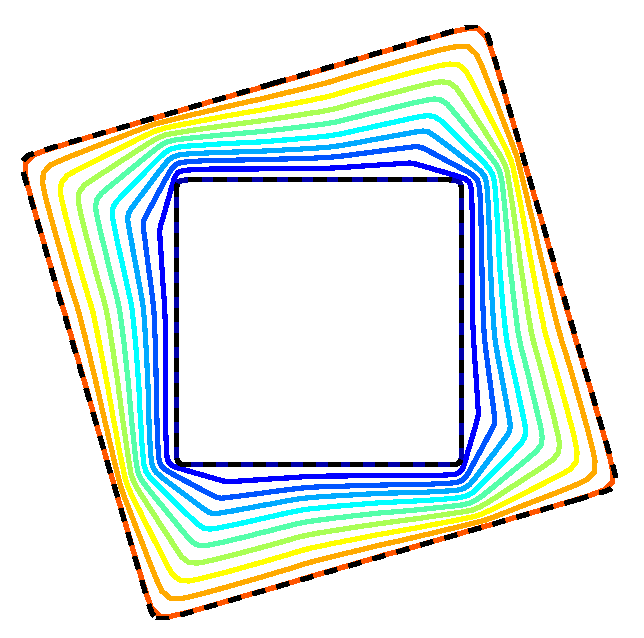
\includegraphics[width=.23\linewidth]{homotopy-bv2-square}&
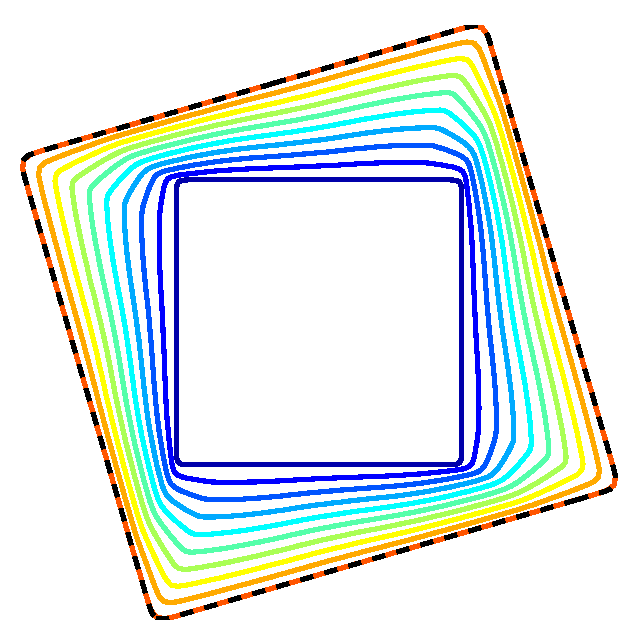
\includegraphics[width=.23\linewidth]{homotopy-sobolev2-square}\\
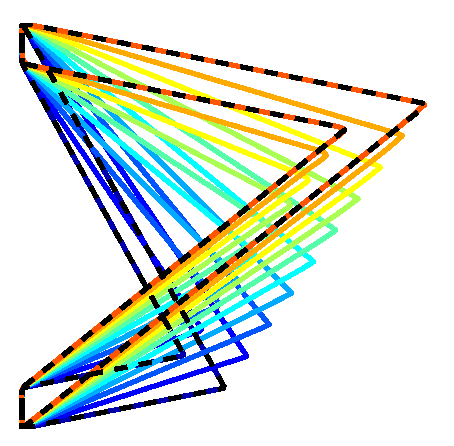
\includegraphics[width=.23\linewidth]{homotopy-bv2-rod}&
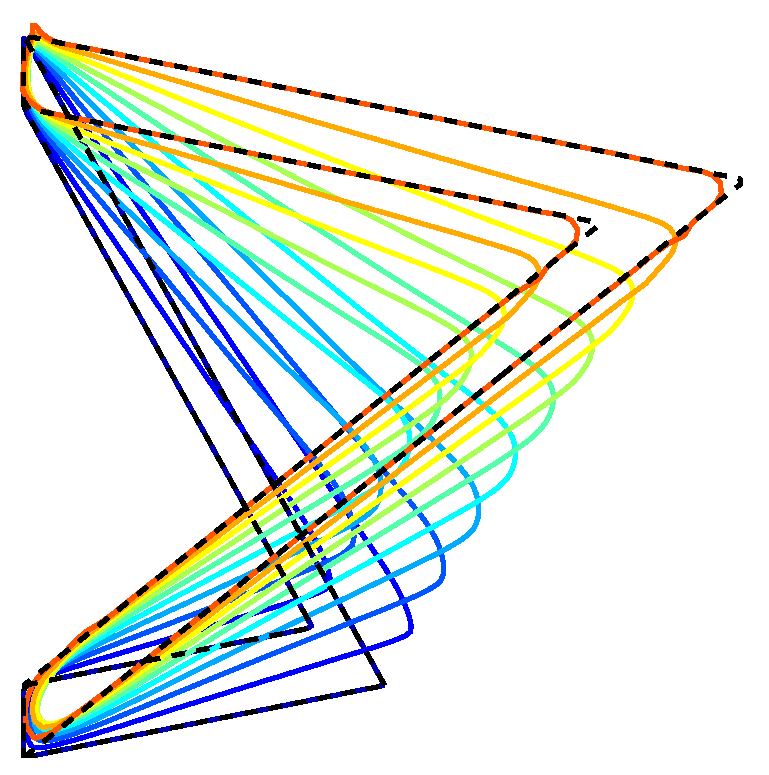
\includegraphics[width=.23\linewidth]{homotopy-sobolev2-rod}\\
$BV^2$ & Sobolev 
\end{tabular}
\caption{\label{geodesics} Homotopies $\Ga^{(\infty)}$ obtained for $BV^2$ Finsler energy (left) and Sobolev metric (right). Each image displays the initial curve $\gm_0$ (black one) and $\gm_1$ (dash line) and the optimal $\{\tilde\GA_{i,\cdot}\}_i$ where the index $1 \leq i \leq N$ is indicated by color variations between blue ($i=1$) and red ($i=N$). \vspace{1mm}}
\end{figure}


Fig.~\ref{geodesics}, top row, shows a simple test case, for which using a trivial constant initialization $\tilde\GA^{(0)}_i = \tilde\gm_0$, for both $BV^2$-and $H^2$-metric, produces a valid homotopy $\Ga^{(\infty)}$ between $\gm_0$ and $\gm_1$.  One can observe that while both homotopies are similar, the Sobolev metric produces a slightly smoother evolution of curves. This is to be expected, since piecewise affine curves are not in the Sobolev space $H^2(\Circ,\RR^2)$. 

Fig.~\ref{geodesics}, bottom row, shows a more complicated case, where using a trivial initialization $\tilde\GA^{(0)}$ fails to give a correct result $\tilde\GA^{(\infty)}$, because the gradient descent is trapped in a poor local minimum. We thus use as initialization the natural bijection $\tilde\GA^{(0)}$, which is piecewise affine and correctly links the singular points of the curves $\gm_0$ and $\gm_1$. It turns out that this homotopy is a stationary point of the energy~\eqref{eq-optim-discrete}, which can be checked on the numerical results obtained by the gradient descent. On the contrary, the Sobolev metric finds a slightly different homotopy, which leads to smoother intermediate curves.

In Fig. \ref{lastone} we show the influence of the choice of  $(\mu_0,\mu_1,\mu_2)$ in \eqref{num-bv2} on the optimization result. We point out in particular the role of $\mu_2$ which controls the jumps of the derivative and is responsible of the smoothness of the evolution.

\begin{figure}[h!]
\centering
\begin{tabular}{@{}c@{\hspace{1mm}}c@{\hspace{1mm}}c@{}}
\includegraphics[width=.25\linewidth]{1,1,00001}&
\includegraphics[width=.25\linewidth]{1,1,001}&
\includegraphics[width=.25\linewidth]{1,1,01}\\
(1,1,10e-05)&(1,1,0.001)&(1,1,0.01)\\
\end{tabular}
\caption{\label{lastone} Finsler $BV^2$-geodesics for different choices of $(\mu_0,\mu_1,\mu_2)$. \vspace{5mm}}
\end{figure}



